\documentclass[../rzero]{subfiles}
\begin{document}
\chapter{Electromagnetism}\label{electromagnetismChapter}

\begin{chapquote}{George Yuri Rainich, 1923\cite{rainichElectrodynamicsGeneralRelativity1925}}
``The electromagnetic field is entirely determined by the curvature of space-time, so that there is no need of further generalizing the general relativity theory.''
\end{chapquote}


\section{What is Electromagnetism}
If you don't know, stop now. Ok, don't stop. It's light and cell phones. 

\section{It's not an 'electric universe'}

Einstein gave a wonderful talk about his ether backtracking in 1920\cite{Einstein1920}, then in 1924 he put out a paper \textit{Concerning the Aether}\cite{einstein1924concerning}(translated version). 

He was annoyed with the success of electricity and magnetism, and how it tilted the field. In my opinion this is still true today, and Einstein's complaints about electromagnetism not being suitable as an '\textit{ether of everything}' (my term I just coined - whaddya think?) are still true. Einstein\cite{einstein1924concerning}:
\begin{quotation}
	There was another way too in which the Maxwell-Lorentz theory set back physicists’ basic understanding. Since electromagnetic fields were seen as fundamental, irreducible entities, they seemed destined to rob ponderable masses, possessing inertia, of their primary meaning. It was shown by Maxwell’s equations that a moving, electrically charged body is surrounded by a magnetic field whose energy is, to first approximation, a quadratic function of speed. It seemed only natural to conceive of all kinetic energy as electromagnetic energy. Thus one could hope to reduce mechanics to electromagnetism, since efforts to reduce electromagnetic phenomena to mechanics had failed. Indeed this looked all the more promising as it became apparent that all ponderable matter was composed of electromagnetic elementary particles. But there were two difficulties that could not be overcome. Firstly the Maxwell-Loretz equations could not explain how the electric charge constituting an electrical elementary particle can exist in equilibrium in spite of the forces of electrostatic repulsion. Secondly electromagnetic theory could not give a reasonably natural and satisfactory explanation of gravitation. Nevertheless the results that electromagnetic theory achieved for physics were so significant they came to be regarded as a completely secured possession, indeed as its most firmly established success.
\end{quotation}

Einstein's facts are still true today:
\begin{itemize}
	\item Electrostatic repulsion is a problem for (QED) particle models.
	\item No gravity from electromagnetism.
	\item Electromagnetism is firmly established as a field.
	\item Electromagnetism is firmly established as a field.
\end{itemize}

You may think you have found a problem in the text - Iv'e gone and duplicated that last point! Sorry, nope. 

\begin{itemize}
	\item Field as a real, base level physical entity.
	\item Field as in a 'what field do you work in?' QFT.
\end{itemize}

Both of these fields are problems for even anyone even trying to mention that electromagnetism might be an emergent phenomenon, which is one reason that there are so few papers on it lately.\cite{barceloElectromagnetismEmergentPhenomenon2014}. There are some that stick out though - from 7 or more decades ago.

\section{Rainich, Misner and Wheeler}

Wheeler pointed out that Einstein also worked on unifying his General Relativty with Electromagnetism, and furthermore that he had no idea of Rainich's work, which seems a shame. Einstein was into altering the equations of General Relativity to include electromagnetism. Wheeler\cite{wheelerCurvedEmptySpaceTime1966}: 

\begin{quotation}
	 Unaware of Rainich's early work, Einstein had tried for many years, up to his death, to invent some new kind of geometry\cite{einstein2003meaning} which would have sufficient richness to describe both gravitation and electromagnetism.
\end{quotation}
	Einstein's non symmetric tensor didn't work. 
	
In contrast, Misner and Wheeler's approach\cite{Misner:1957mt}\cite{Wheeler1957quantumGeo}, based on Rainich\cite{rainichElectrodynamicsGeneralRelativity1925} does exactly what I am aiming at here, with one exception - Misner and Wheeler obtain 'charge without charge' from field lines trapped in wormholes. 

I instead try to construct a wormhole free\footnote{I like wormholes as much as the next person, don't @ me.} source of  electromagnetism. With such a construction, much of the rest of 'already unified' formalism of Rainich, Misner and Wheeler can be used.

\section{Electromagnetism from General Relativity}
Here is the part where I get to do the physics equivalent of pulling a rabbit out of a hat. Everyone \textit{knows} that since electromagnetism is so much stronger than gravity, my task here is not merely hopeless. So let's see just how funny (in at least three senses of the word) we can get in this chapter. 


\section{Emergence}
The emergence of electromagnetic phenomena from General Relativity comes from starting at an electron model. Since an electron is a spinning thing, with known mass and angular momentum, I start with the known General Relativity solution for a spinning thing with mass, the  solution found in 1963 by Roy Kerr\cite{kerrGravitationalFieldSpinning1963}. I don't use the Kerr - Newman 'charged' solution\cite{newmanNoteKerrSpinningParticle1965}, after all I am attempting to get electromagnetism to emerge from General Relativity, so I can't just toss electrical stuff in there at the outset, right? Burinskii\cite{Burinskii2008} and others have employed Kerr Newman solutions as possible models for the electron, but, as I stated, I'm not using built in charge. I am attempting to construct charge from gravtitational phenomena.

Other people have looked at electron as a Compton radius ring of some sort. Usually called zitterbewegung motion from the Dirac equation\cite{diracQuantumTheoryElectron1997}. See Hestenes\cite{Hestenes1990}, Barut\cite{Barut1984}, and Maddox\cite{Maddox1987} (yes the editor of Nature back in the day, when Nature meant something).

The Kerr solution for a particle of the same mass and spin as an electron is known in the biz as a 'naked singularity', which is a thing that 99$\frac{44}{100}$\% of pure physicists know can't exist in nature. But they won't argue that this naked ring is a solution of Einsteins vacuum equations, (i.e. equation (\ref{vacuumEquation})). So yes, we are going to have to throw caution to the wind here and just assume that the Kerr solution (or something like it as we will see in chapter \ref{electronModelChapter}) is a possible model of the electron. 

As a defence of my so far nascent electron model, I will point out that there is no truly self consistent model of the electron known at this point. As the Richard Feynman one of a few authors of QED, our best 'standard physics' model of the electron pointed out\cite{Feynman1985} (page 127): 

\begin{quotation}
"The shell game that we play to find n and j is technically called “renormalization.” But no matter how clever the word, it is what I would call a dippy process! Having to resort to such hocus-pocus has prevented us from proving that the theory of quantum electrodynamics is mathematically self-consistent. It’s surprising that the theory still hasn’t been proved self-consistent one way or the other by now; I suspect that renormalization is not mathematically legitimate." 
\end{quotation}

Our standard model physicist\footnote{A \textit{standard model physicist} is a normal card carrying member of the professional ranks of the academic industrial complex, level 3 or higher.} will tell you that renormalization isn't a problem - and they are right - but only because so many worse problems have arisen in theoretical physics over the past seven decades since QED\cite{feynmanSpaceTimeApproachQuantum1949}. QED renormalization is now a walk in the park. To be fair, it does actually work. (Although see Consa\cite{Cioletti2006} for a negative outlook on the QED industry.)

Basically, the problem in all electron models, including QED, is quite simple to elucidate: the electron explodes when you try to assemble a model from \textit{charge paste} - the energy you need to bring together bits this paste to form a small thing that looks like an electron goes to infinity. The problem is that each bit repels all the other bits as you try and squeeze it all into one place. I'll go into this more in chapter \ref{physicsTodayChapter}.  

This Kerr naked singularity turns out to be very long (some $10^{42}$ longer than the natural 'black hole' size of the electron). Dividing this long singularity into  $10^{42}$ sections, I find that each section has a gravitational wave interaction about equal to the gravitational Newtonian interaction between two electrons (a cross section). And all these small interactions can add up to a huge Coulomb level force between two of them.  

\subsection{How to add it up}
The expression for the electromagnetic Coulomb force $F_e$ between two electrons is 

\begin{equation}\label{coulomb_force}
	F_e = k_e\frac{q^2}{r^2} = \pm \frac{\alpha \hbar c}{r^2}.
\end{equation}

The second version is for single point charges only. It is a more fundamental way of looking at electromagnetism, since in reality all charges are of unit size. I will use this second one. Note that:

\begin{itemize}
  \item $\alpha$ is a number, about 1/137.\footnote{Feynman - "all good theoretical physicists put this number up on their wall and worry about it."\cite{Feynman1985} (I doubt they do any longer --Tom) }
  \item $\hbar$ is the famous quantum constant.
  \item $c$ is the speed of light.
  \item $r$ is the distance between the two electrons.
\end{itemize}

For for the force of gravity $F_g$ we have

\begin{equation} \label{grav_force}
	F_g = G\frac{m_e^2}{r^2}.
\end{equation}

Where

\begin{itemize}
  \item $G$ is Newton's gravitational constant.
  \item $m_e$ is the mass of the electron.
  \item $r$ is the distance between the two electrons.
\end{itemize}

The large, famous value of the ratio between these two forces, which I will call $k'$ is by inspection of eqn (\ref{coulomb_force}) and (\ref{grav_force})

\begin{equation} \label{electric_ratio}
	k' = ratio_{electric} = \frac{k_e q_e^2}{G m_e^2} = \frac{\alpha \hbar c}{G m_e^2} = \num{4.166e42}
\end{equation}


I will now construct a force $k'$ stronger than the usual Newtonian gravitational force using only the Kerr solution of Einsteins equations, with no reference to electromagnetism. If your afraid of magicians, look away, now.

\section{The Kerr Singularity with Electron Parameters}
The well known Kerr solution of Einsteins equations has a naked ring singularity for $J/mc > Gm/c^2$, somewhat better known as $a > m$ in geometric units. I use SI units in this section. In Kerr-Schild coordinates (a coordinate system that is Minkowskian almost everywhere)\cite{Visser2008}, the expression for the location of the ring singularity is $x^2 + y^2 = (J/mc)^2$, (avoiding the use of r, as r has a meaning on its own in the Kerr solution in Kerr-Schild coordinates). Using the measured experimental values for the mass $m_e$ and spin angular momentum $\hbar/2$ of an electron, the radius of the ring singularity is:
\begin{equation} \label{radius_eqn}
	R_{ring} = J/mc = \hbar/2m_ec = \num{1.93e-13}m
\end{equation}

Thus the ring singularity is 0.5 of the Compton wavelength in circumference. This is a \textit{huge} radius, and I will go into how this sort of thing might be possible in chapter \ref{electronModelChapter}. This radius can also be calculated as a ratio. The obvious other gravitational length to compare it to is the Schwarzschild radius $r_s = 2Gm_e/c^2$ for the electron mass, we get a ratio of these sizes:

\begin{equation}
	size \ ratio = \frac{\hbar/(2m_ec)}{(2Gm_e/c^2)} = \frac{\hbar c}{4G m_e^2} = \num{1.4e44}.
\end{equation}

 It is noteworthy that this ratio is already very close to the ratio $k'$ of the strength of the electric Coulomb force to the gravitational attraction between two electrons. Indeed, multiplying this ratio by the four times the fine structure constant (i.e. $\approx 0.029 $ ) gives one \textit{exactly} $k'$ - the ratio of the electric and gravitational force on two electrons:
 
\begin{equation}
	ratio = 4\alpha \frac{\hbar/(2m_ec)}{(2Gm_e/c^2)} = \frac{\alpha \hbar c}{G m_e^2} = \num{4.166e42} = k'.
\end{equation}


These are of course the same arrangement of constants as in (\ref{electric_ratio}). The difference here is that this ratio is now calculated without any references to the electric Coulomb force. It is simply a ratio of the radius of a Kerr singularity of the electron's mass and spin angular momentum to that of Schwarzschild radius for the electron mass $r_s$, along with a factor of $4\alpha$ added in by hand (see the next section). 

Things are getting interesting, but we're not there yet. What we have is a ring that measures $\num{1.4e44}$ times the size of an un-spinning black hole the mass of an electron. The next question is how do two of these rings a distance $r$ apart interact strongly? In other words - I have some compelling (to me) geometry - but no force yet. 


\section{Gravitational Waves as carriers}

%There is a connection between the size of the Kerr ring singularity as measured in units of the electron Schwarzschild radii($r_s$) to the effect of Coulomb repulsion. Can charge itself be constructed of nothing more than geometry? The mere calculation of the ratio does not give one a recipe for how electromagnetism can be constructed from general relativity, but there are some hints at a mechanism.
\begin{figure}\label{kerr-electric-image}
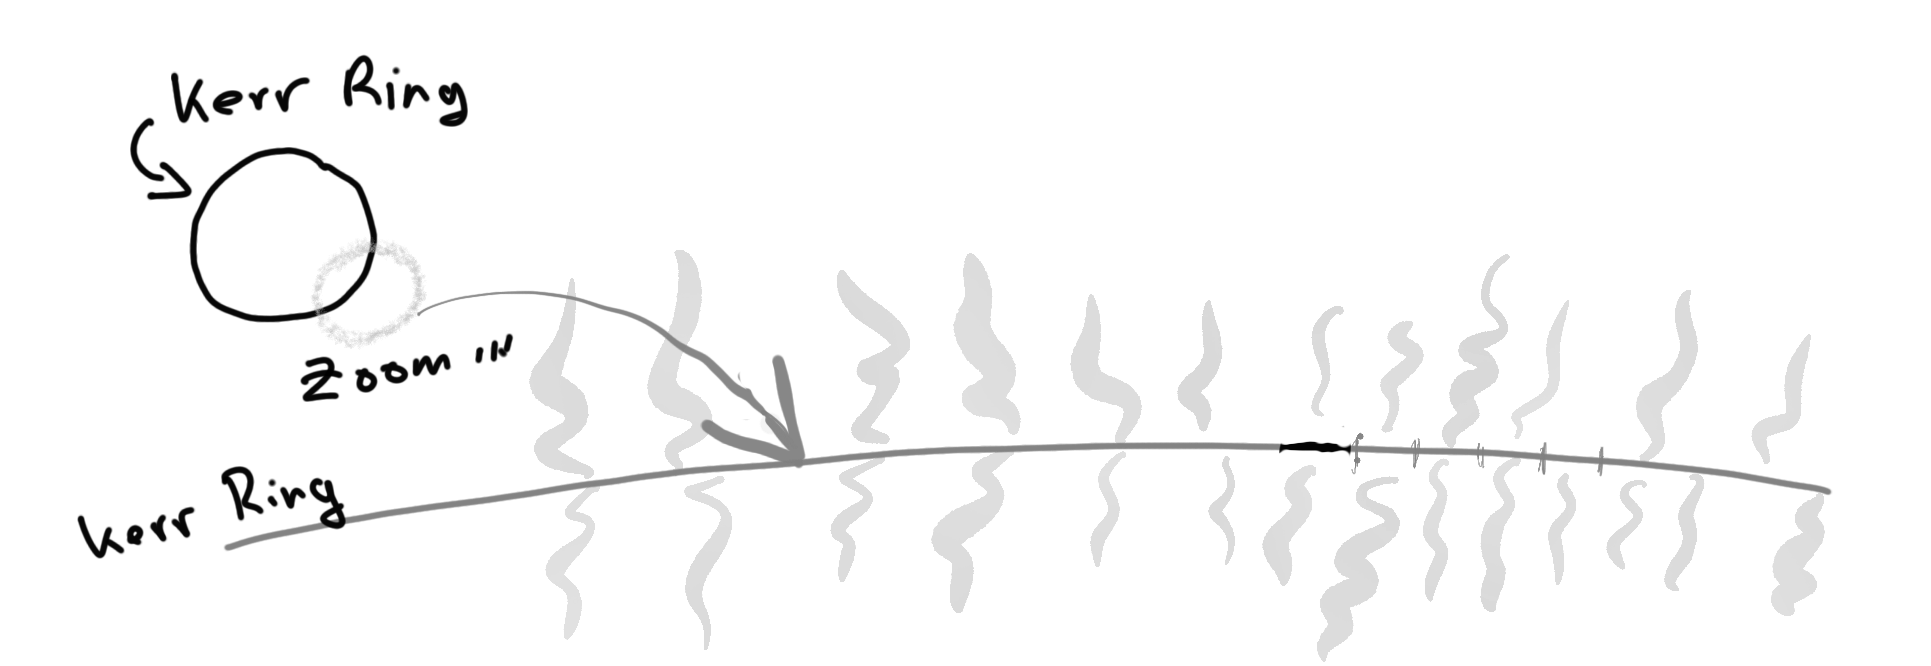
\includegraphics[width=0.99\textwidth]{chapters/images/kerr-electric.png}
\caption{Upper left: A Kerr ring singularity. Main: zoom in on a small section of it to reveal gravitational waves of a wavelength equal to the Schwarzschild radius (and up). This results in about $\num{1.4e44}$ segments, each interacting with an $\alpha$ cross section.}
\end{figure}



 If one imagines the ring singularity is cut into $\num{1.4e44} $ pieces each of size $r_s$ and each piece interacts with the nearby electron with a 'gravitationally sized' force on each section of $\alpha G m_e^2/r^2 $, perhaps one can create electromagnetic strength forces from entirely gravitational means. $4\alpha$ then is perhaps some scale factor/antenna cross section of 'order 1' (well $ 0.029$).
   
 How can a single section of the ring with a tiny mass of $ 10^{-44}m_e $ and length $r_s$ interact so strongly? The answer might lie in gravitational wave interaction, it better, because that's all I really have, as the point of this book is to build physics with nothing but General Relativity.  It seems that the properties of a singularity are such that it will interact very well\cite{Nakamura1993} with gravitational waves. A gravitational wave effect could thus be strong enough to provide a net force of $\alpha G m_e^2/r^2 $ per segment, with super radiance and absorption taken into account. For comparison, an astrophysical black hole of radius $r_s$ can, via superradiance, emit or absorb a significant fraction (~10\%!) of its energy given the right gravitational wave parameters.\cite{Brito2015}.  
  
 Each section would need to be interacting with gravitational waves of a fantastic frequency - the wavelength would have to about match the Schwarzschild radius ($r_s$) of the electron. This is of course a frequency well beyond that usually conceived in accepted quantum physics - but remember - I am trying to also emerge quantum mechanics from General Relativity, so I'm asking you to sit on this 'annoyance' for a while (until chapter \ref{quantumMechanicsChapter}).  In for a penny and all that.
 
 The amplitude of the gravitational waves at this incredible, $10^{65} Hz$ frequency would be tiny, as the energy carried in a gravitational wave depends on  amplitude and square of frequency, much too small to cause directly measurable 'gravitational' effects. These waves are  many orders of magnitude smaller in amplitude than those measured by LIGO, for example. We would only see the force of one electron on another as they exchange gravitational wave energy, interpreting it as the Coulomb force, since there are so many interactions happening at once. 
 
 Once we have individual segments interacting with the right force we have recreated the Coulomb force, or at least a rough mechanism as to how it would work. Another way of thinking of it is to look at the overall energy balance - the waves configuration of two electrons will drop in energy as the two electrons move further apart from each other. 
 
 
 Other researchers have looked at models of electromagnetic interaction - Cetto\cite{Cetto2013} outlines a physical description of QED, using a physical model of QED arising from a stochastic background field. 
 
 We're still at the 'believe me' level here, and it's going to stay that way. I leave it to someone to point out all the problems with this kind of solution. But there are some good points:
 
 \begin{itemize}
 	\item Not a QED like charged goo model.
 	\item Fewer infinities (there is that naked singularity).
 	\item Easy to understand for engineer types.
 \end{itemize} 

 
 \section{Carrier waves} 
 Essentially, electromagnetic waves - photons are constructed as modulations of these fundamental gravitational waves - the gravitational waves are carrier waves. In this model, spin 1 is simply a result of moving a charge up and down. The carriers are 'spin 2'.
 
 If you think you know that spin 1 photons can't be built with spin - 2 gravitational waves, I have news for you. Here, for instance is someone\cite{shiObservationAcousticSpin2019} building spin 1 from a scalar (pressure wave) acoustic field. Basically, you get spin 1 by taking a source exchanging energy and wiggling it up and down. Another source/receptor will see the other source and vibrate up and down in the same direction. The experimentally observed spin of a field can be emergent. As an example Cetto de la Peña obtain fermion statistics from a spin one field.\cite{cettoElectronSystemCorrelated2016}. Here Barceló\cite{barceloElectromagnetismEmergentPhenomenon2014} shows how one might emerge electromagnetism itself. Also see Ranada\cite{ranadaTopologicalTheoryElectromagnetic1989}.
 
 The idea is to use this fundamental energy exchange via gravitational waves as a carrier wave for electromagnetic waves. An EM wave is thus composed of trillions of trillions of gravitational carriers - underneath it, so to speak. 
 
 I am going to need to expand this, get some drawings going, etc. 
  
  Lorentz + Coloumb == EM. 

 \section{Calculating \texorpdfstring{$ \alpha $}{Alpha}} 
 The hypothesis that these ultra high gravitational waves 

\section{The End (of this chapter)}
The ratio of the size of the Kerr solution to the Schwarchild solution for an electron being the same as the ratio of electric to gravtiational forces is telling.

The 


\end{document}
